\documentclass[a4paper,12pt]{article}

\usepackage[utf8]{inputenc}
\usepackage[T1]{fontenc}
\usepackage{lmodern}
\usepackage[polish]{babel}
\usepackage{geometry}
\geometry{a4paper, top=2.2cm, bottom=2.2cm, left=2.5cm, right=2.5cm}

\usepackage{amsmath,amssymb}
\usepackage{booktabs}
\usepackage{graphicx}
\usepackage{float}
\usepackage{caption}
\usepackage{multirow}
\usepackage{array}
\usepackage{xcolor}
\usepackage{hyperref}
\usepackage{siunitx}
\sisetup{output-decimal-marker={,}, locale=DE}
\usepackage{parskip}
\setlength{\parskip}{4pt}

\graphicspath{{wyniki_pomiarow/}}

\title{}
\date{}

\begin{document}

\begin{titlepage}
\centering
{\Large Sprawozdanie nr 1 (Seria 2)\\[6pt]}
{\LARGE \textbf{Propagacja wiązki gaussowskiej na granicy ośrodków}\\[18pt]}

\begin{tabular}{@{}ll@{}}
\textbf{Przedmiot:} & Fotonika \\
\textbf{Data wykonania ćwiczenia:} & 04.05.2026 \\
\textbf{Prowadzący:} & Mgr. Inż. Eliza Miśkiewicz \\
\textbf{Skład zespołu:} & 1. Kamil Suchy \\
\textbf{Grupa:} & TI-L1 \\
\textbf{Zespół:} & Z5 \\
\end{tabular}

\vfill
\noindent\textbf{Podpis prowadzącego:} \hrulefill
\end{titlepage}

\section{Wstęp teoretyczny}
Wiązka gaussowska jest rozwiązaniem równań Maxwella w przybliżeniu paraksjalnym,
którego profil natężenia w przekroju poprzecznym ma kształt funkcji Gaussa.
Jej geometrię opisują m.in. długość fali $\lambda$, promień przewężenia $w_0$,
położenie przewężenia $z_0$ oraz odległość Rayleigha $z_R = \pi w_0^2/\lambda$.
Ważnym parametrem jest zespolony parametr wiązki $q(z) = z - i z_R$.
Transformacja wiązki przez układ optyczny opisywany macierzą ABCD ma postać:
\begin{equation}
q'(z) = \frac{Aq(z) + B}{Cq(z) + D}.
\end{equation}
Niezmiennikiem wiązki jest iloczyn promienia przewężenia i kąta rozbieżności:
$w_0\theta = \lambda/\pi$.

Dla sferycznego frontu fali przechodzącego przez sferyczną granicę o promieniu
$R_S$ pomiędzy ośrodkami o współczynnikach załamania $n_1$ i $n_2$ zachodzi zależność:
\begin{equation}
\frac{n_2}{R_2} = \frac{n_1}{R_1} + \frac{n_2 - n_1}{R_S},
\end{equation}
co można zapisać w postaci $R_2 = n_2 R_1 / (1 + D R_1)$, gdzie
$D = (n_2 - n_1)/R_S$. W ćwiczeniu przyjęto $n_1 = 1$ oraz wartości domyślne:
$\lambda = 1{,}0$, $n = 3{,}5$, $R_1 = -4$, $R_S = 4$.

\section{Wykresy pomiarowe}
Poniżej zamieszczono wykres dla wartości domyślnych parametrów symulacji, zgodny
z oczekiwanym wynikiem referencyjnym.

\begin{figure}[H]
\centering
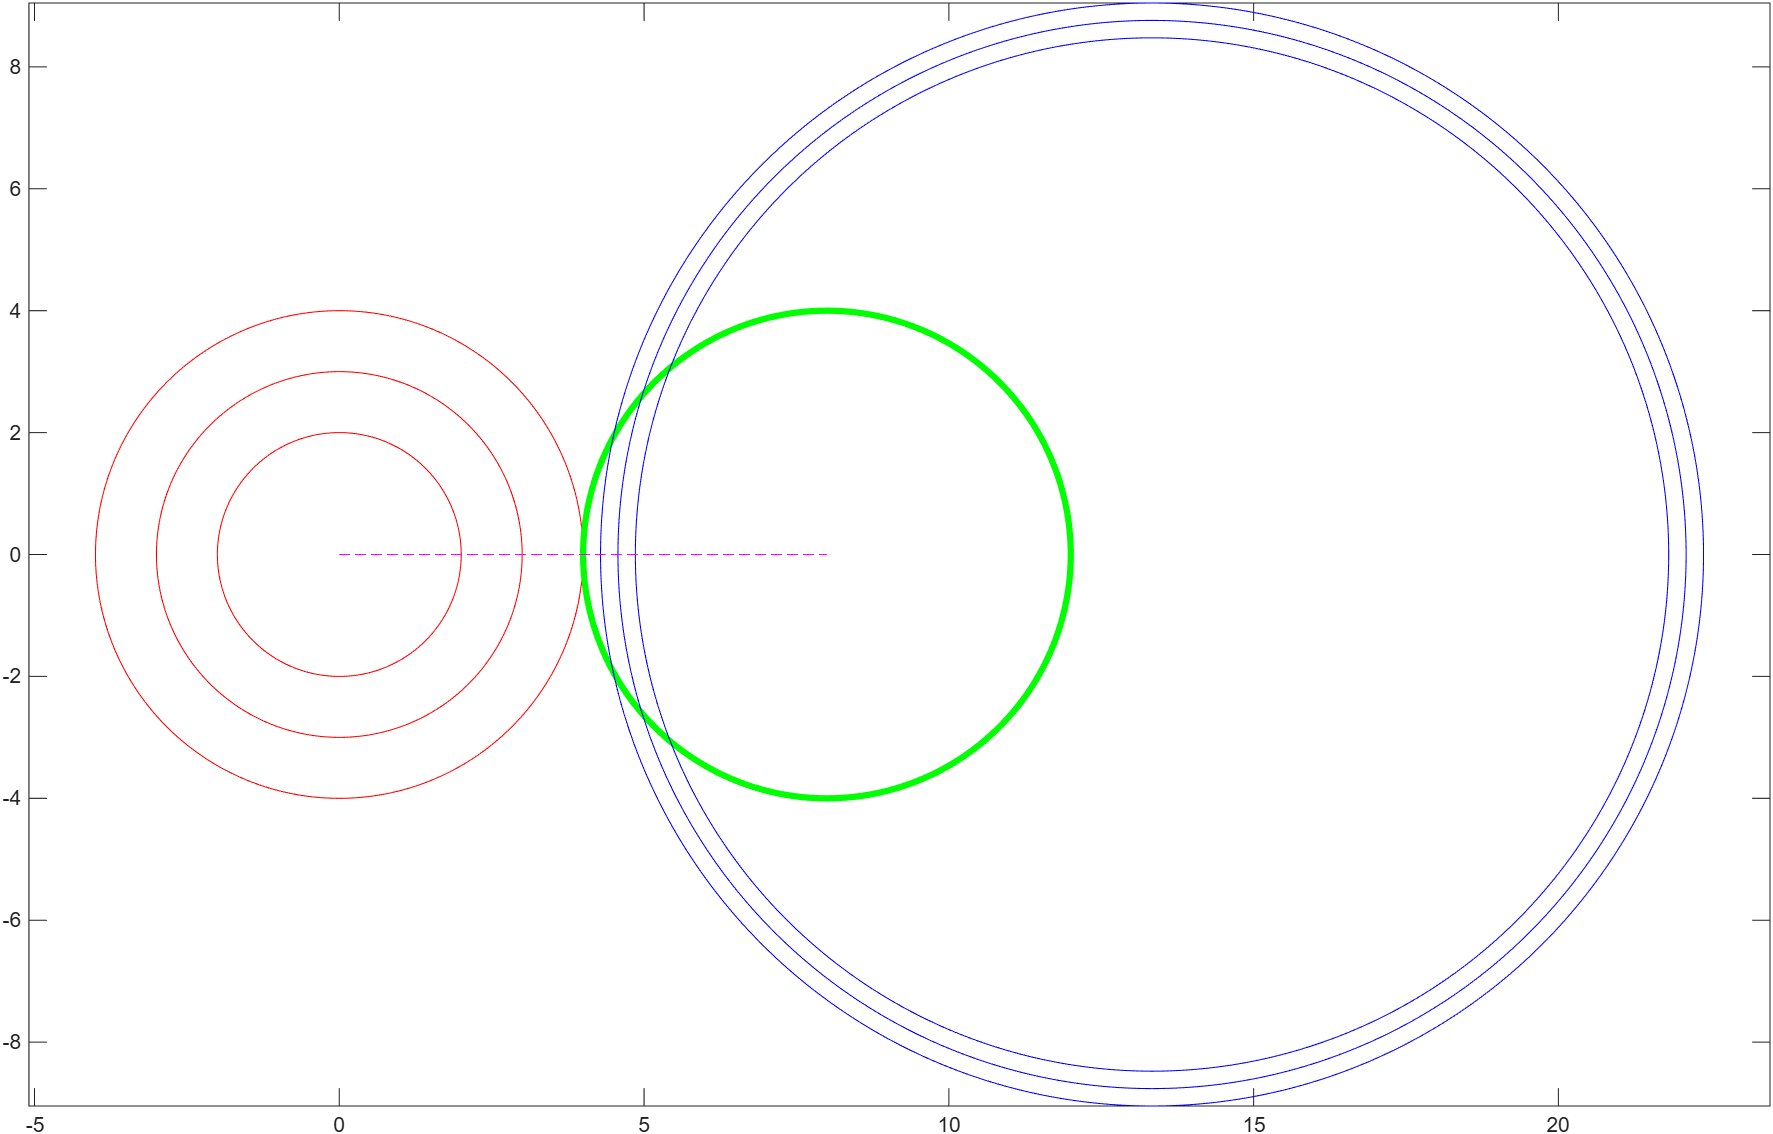
\includegraphics[width=0.8\textwidth]{wykres_domyslny.png}
\caption{Wykres dla wartości domyślnych: $\lambda=1{,}0$, $n=3{,}5$, $R_1=-4$, $R_S=4$.}
\end{figure}

\section{Wykresy z symulacji}
Dla każdej serii zmian parametrów zaprezentowano porównanie skrajnych wartości,
aby uwidocznić wpływ parametru na krzywiznę i gęstość frontów falowych.

\subsection{Zmiana długości fali $\lambda$}
\begin{figure}[H]
\centering
\begin{minipage}{0.48\textwidth}
\centering
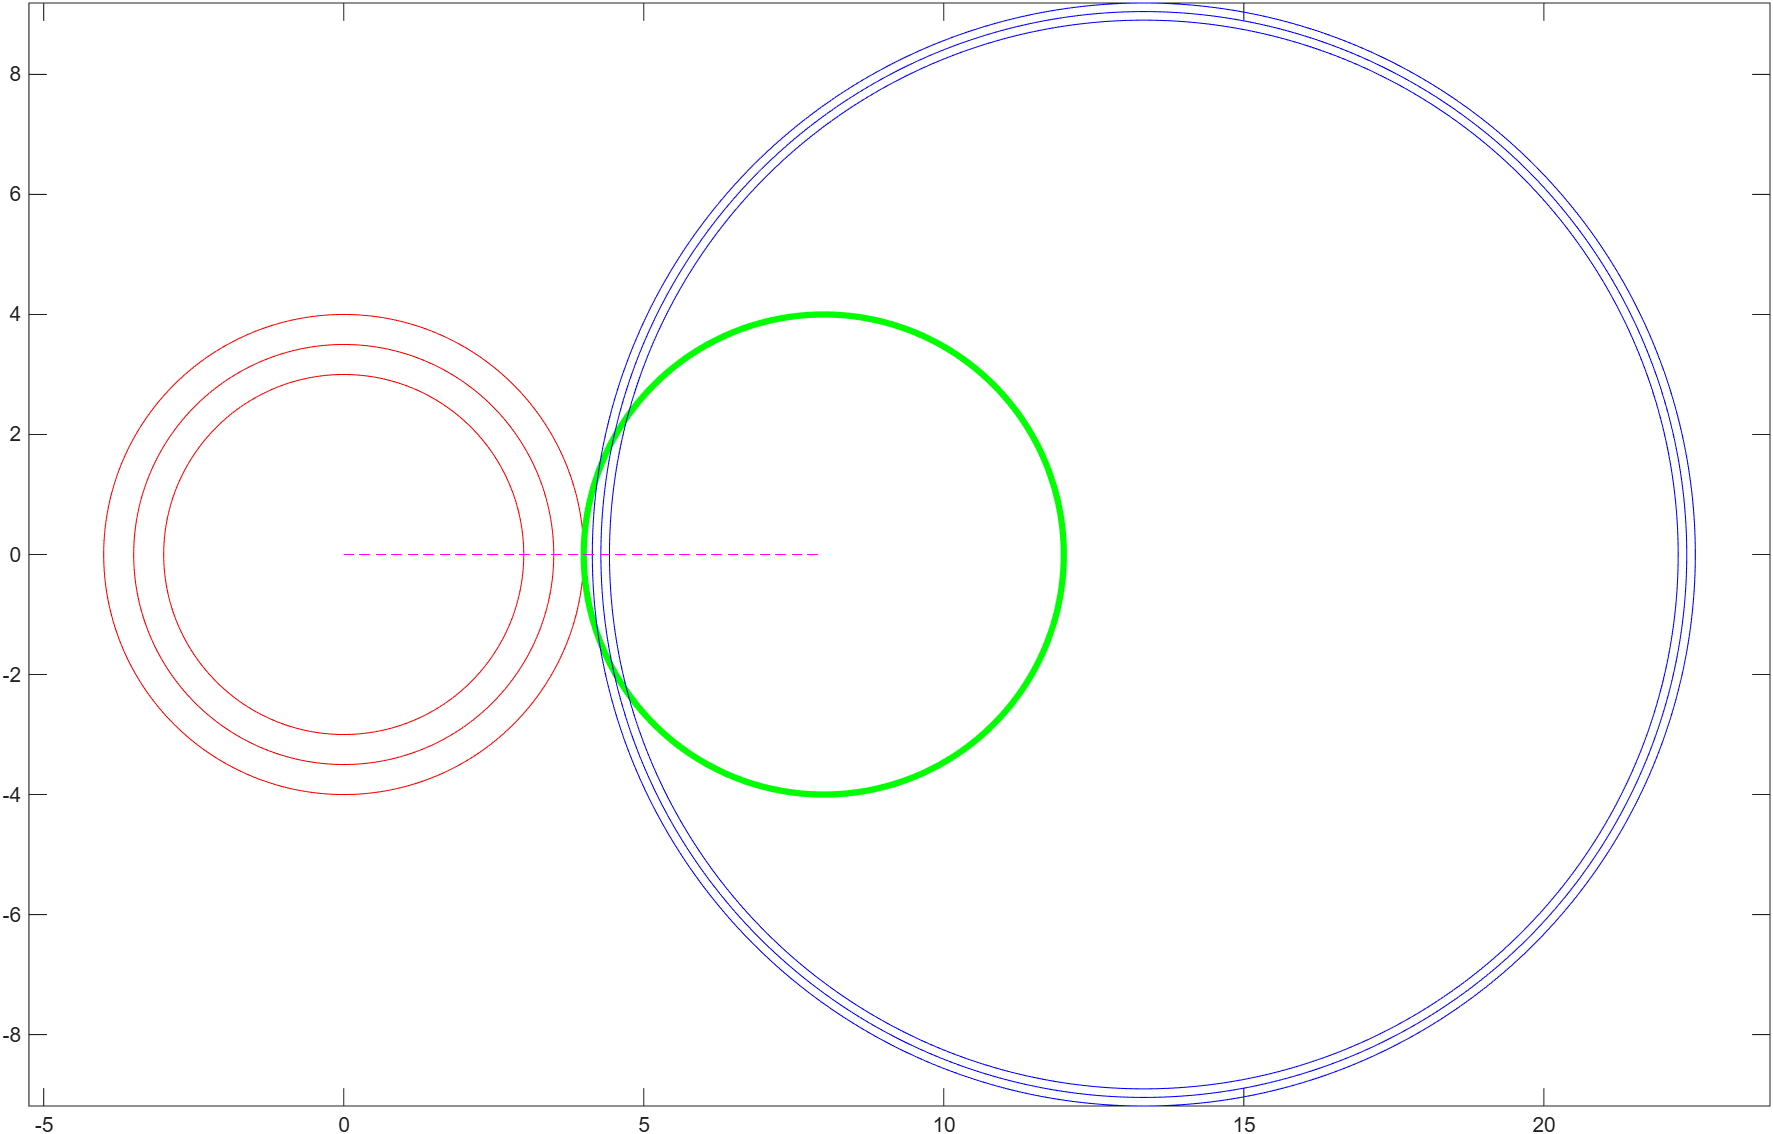
\includegraphics[width=\textwidth]{lambda=0,50.png}
\textit{(a) $\lambda=0{,}50$}
\end{minipage}
\hfill
\begin{minipage}{0.48\textwidth}
\centering
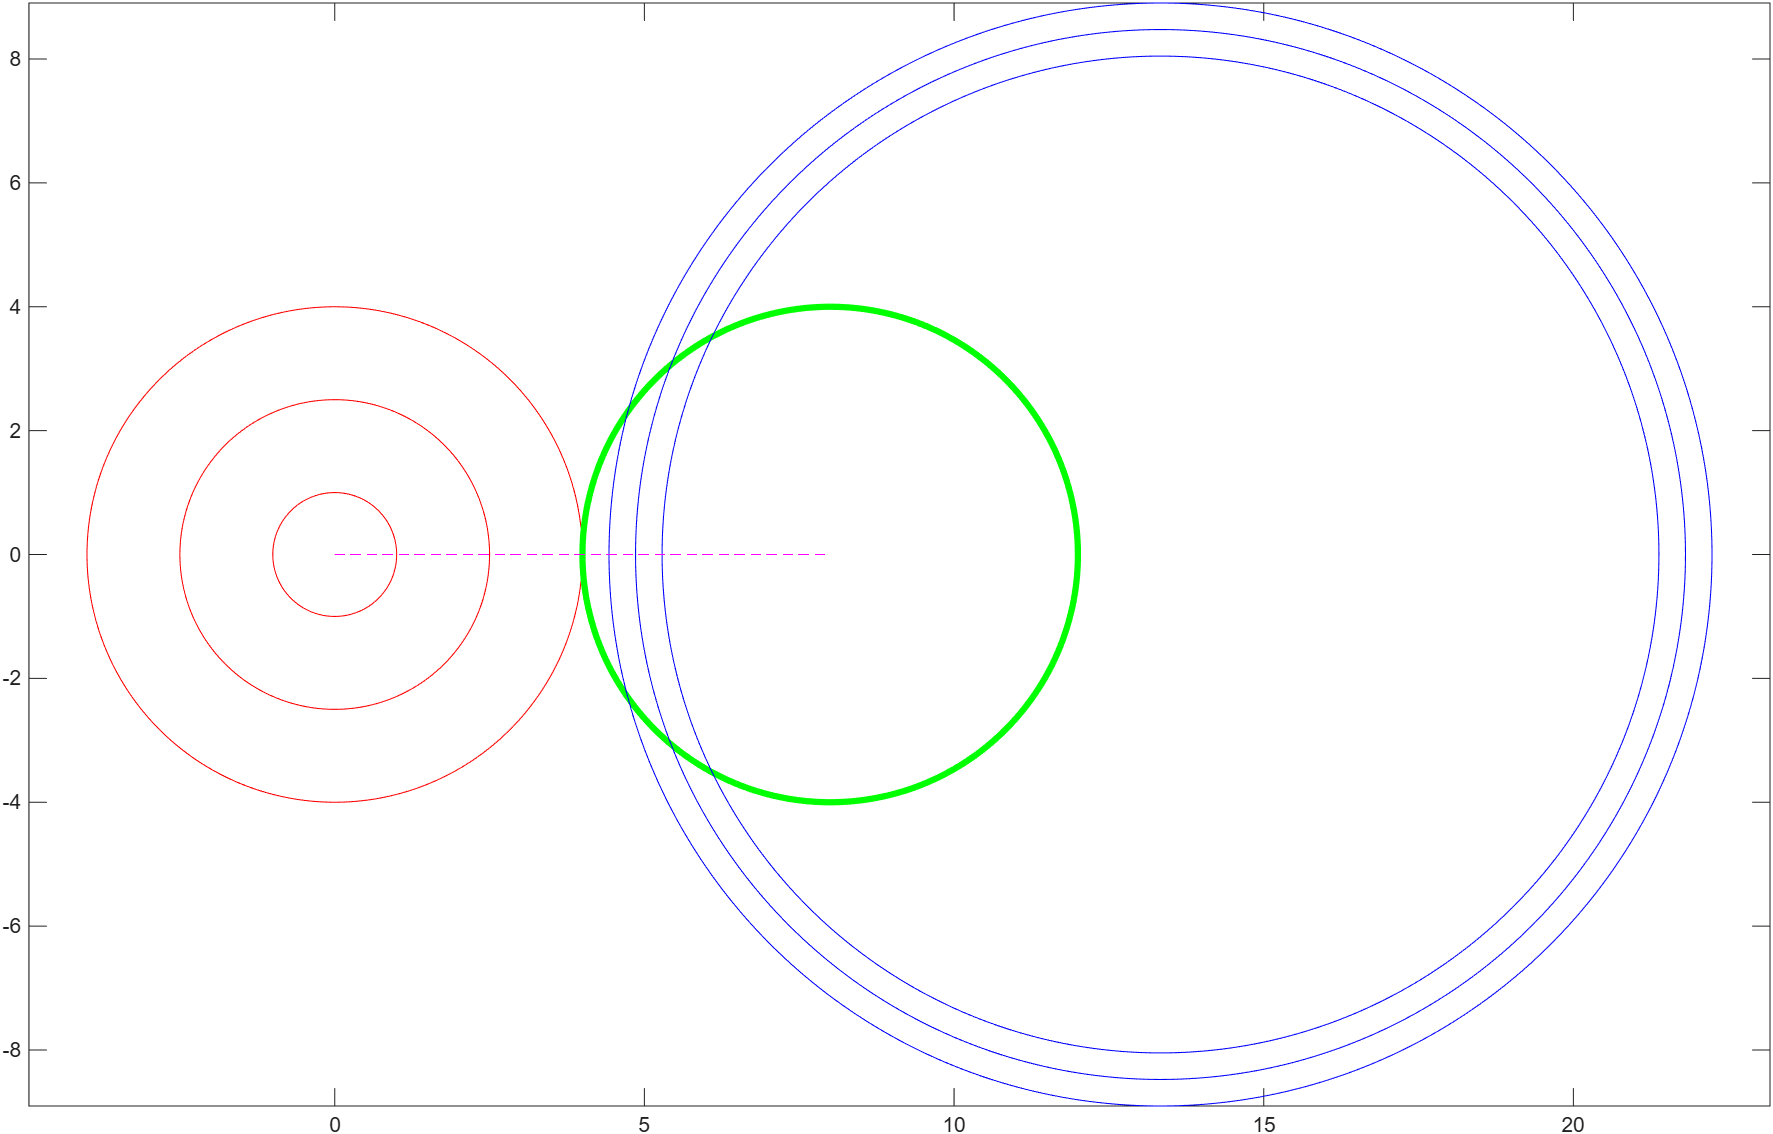
\includegraphics[width=\textwidth]{lambda=1,50.png}
\textit{(b) $\lambda=1{,}50$}
\end{minipage}
\caption{Wpływ długości fali na odstęp między frontami.}
\end{figure}

\subsection{Zmiana współczynnika załamania $n$}
\begin{figure}[H]
\centering
\begin{minipage}{0.48\textwidth}
\centering
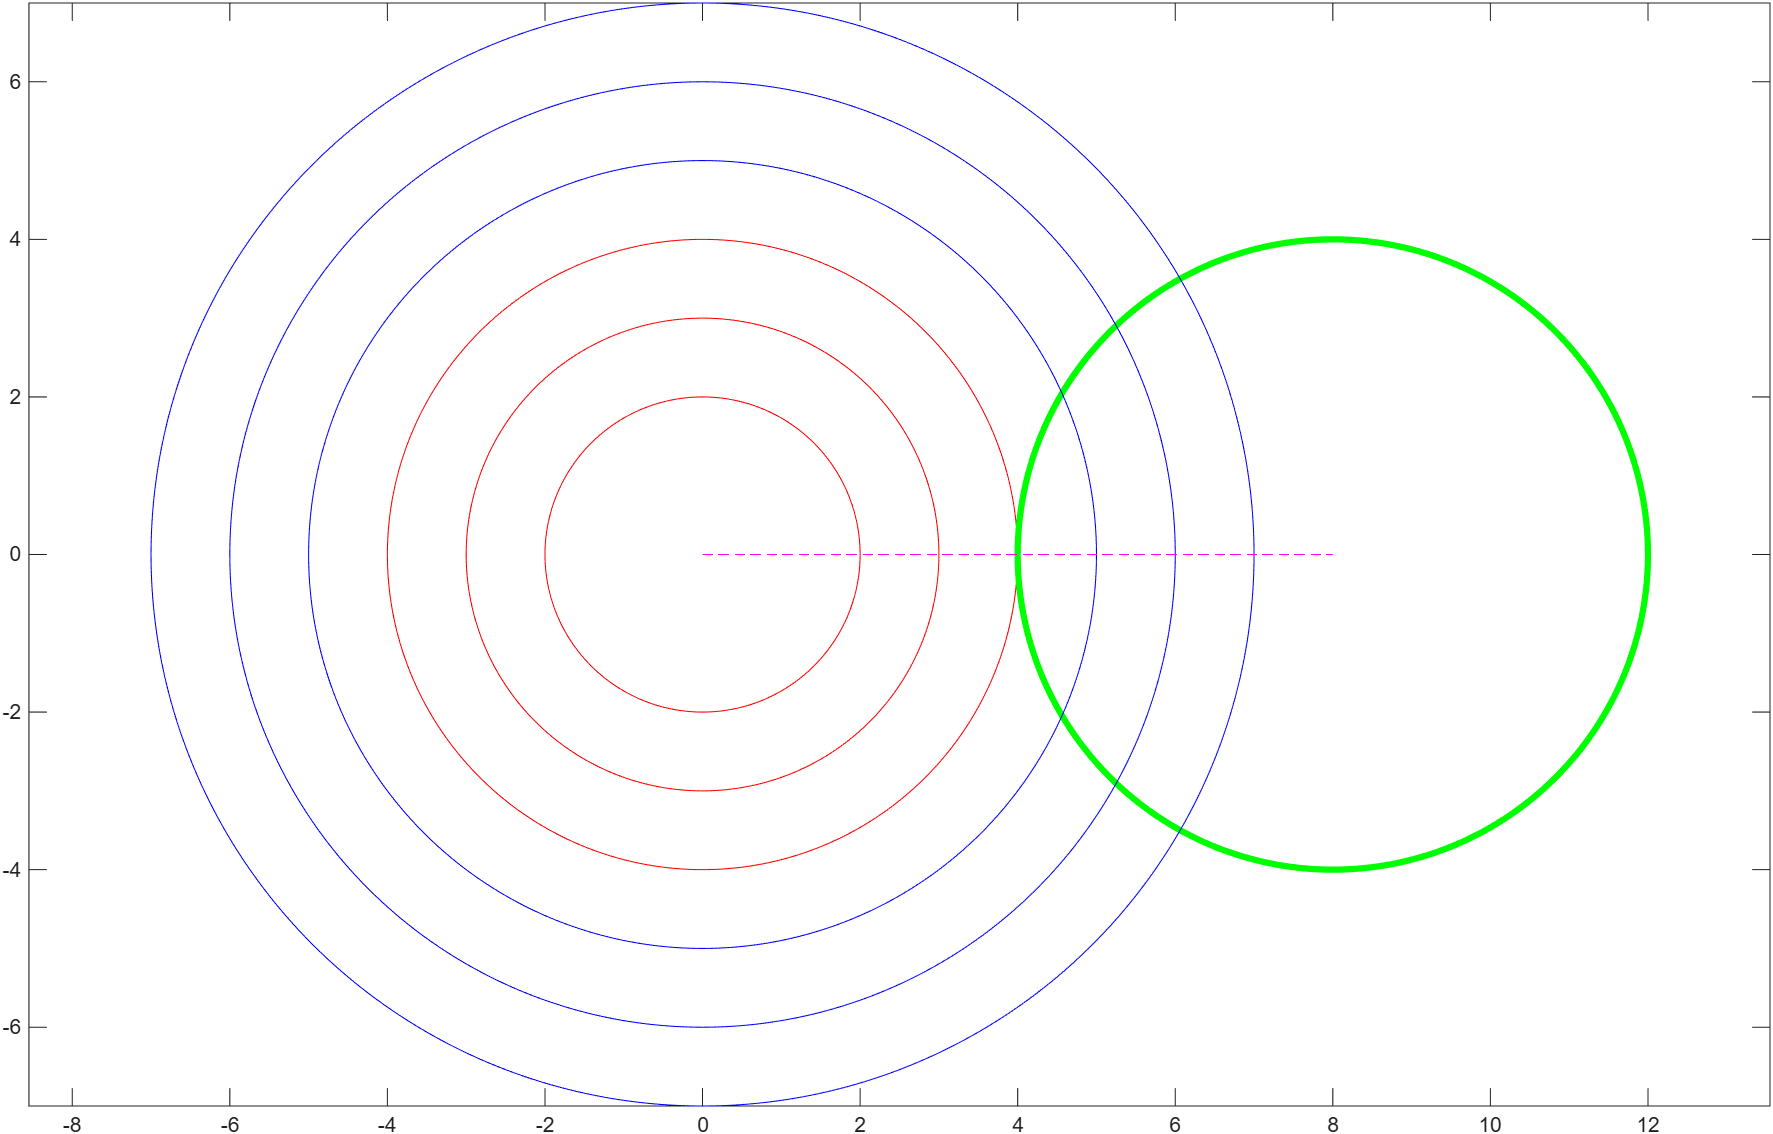
\includegraphics[width=\textwidth]{n=1.png}
\textit{(a) $n=1{,}00$}
\end{minipage}
\hfill
\begin{minipage}{0.48\textwidth}
\centering
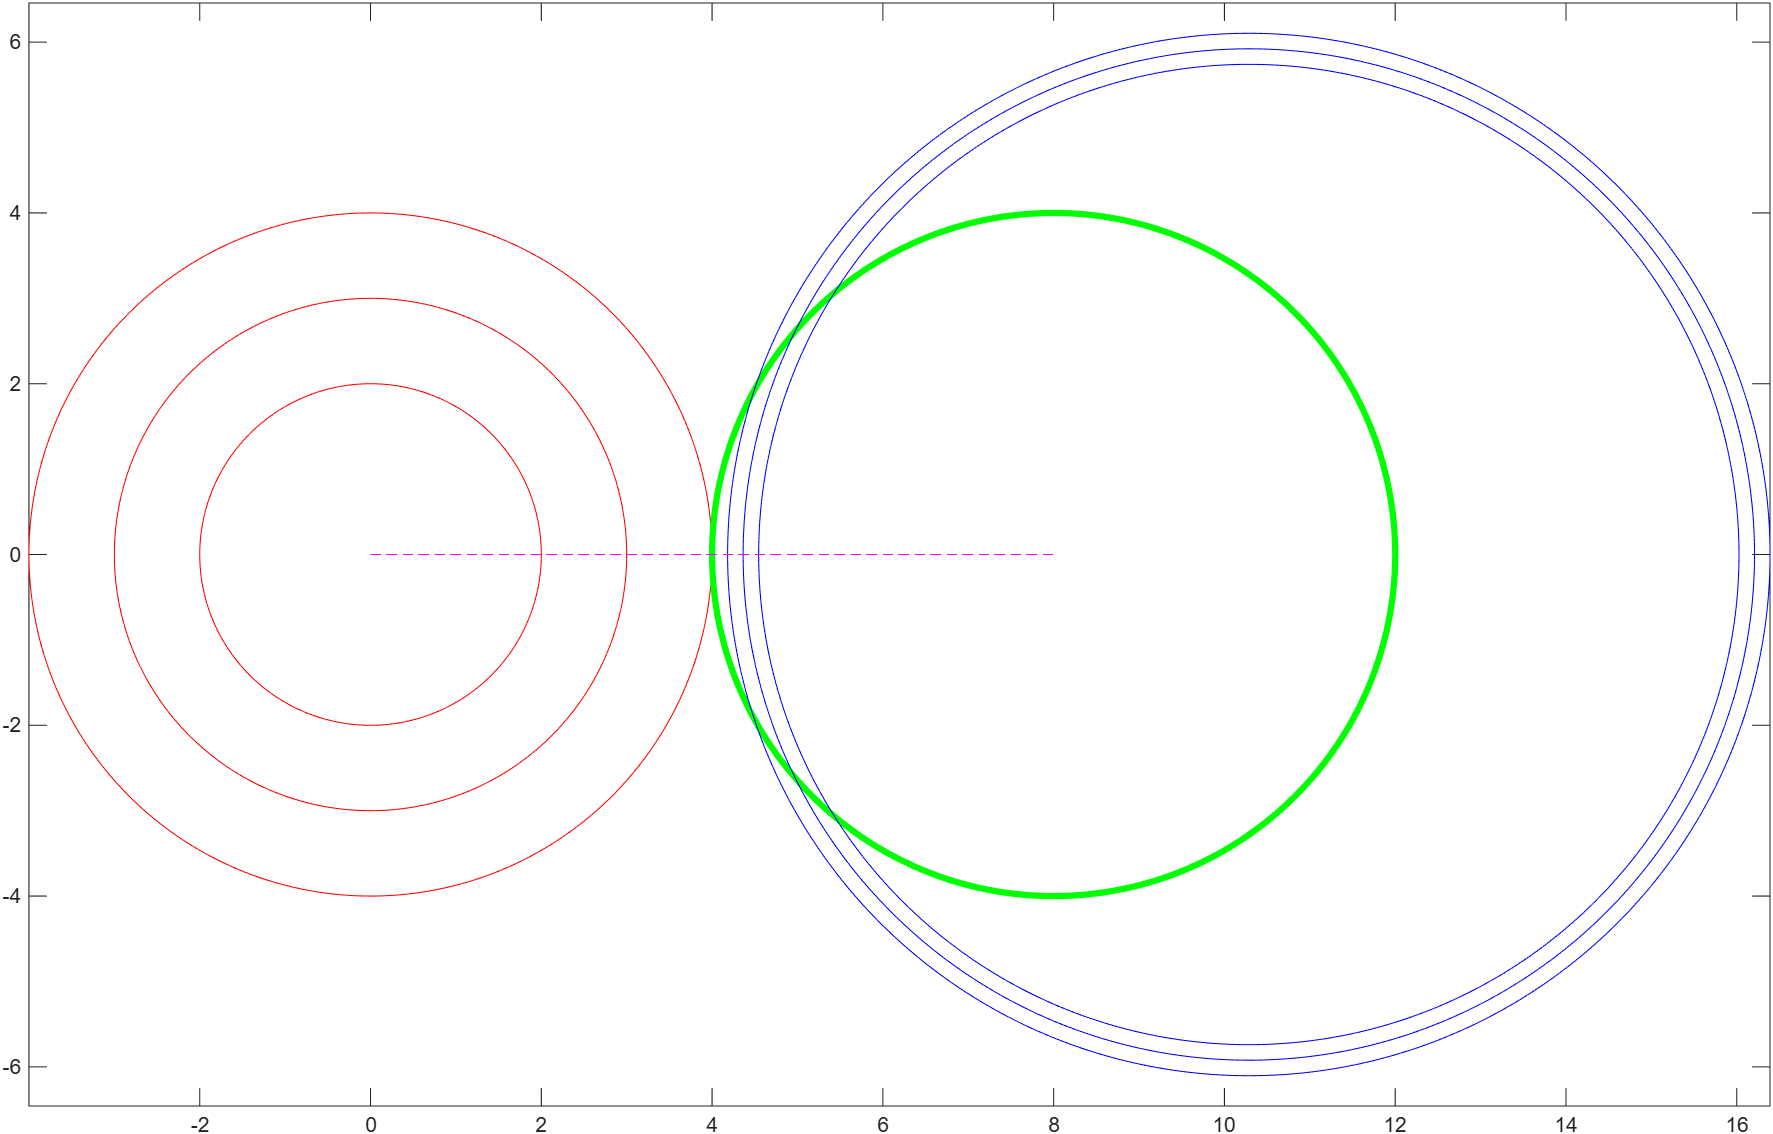
\includegraphics[width=\textwidth]{n=5,50.png}
\textit{(b) $n=5{,}50$}
\end{minipage}
\caption{Wpływ współczynnika załamania na krzywiznę frontu w ośrodku 2.}
\end{figure}

\subsection{Zmiana promienia krzywizny frontu wejściowego $R_1$}
\begin{figure}[H]
\centering
\begin{minipage}{0.48\textwidth}
\centering
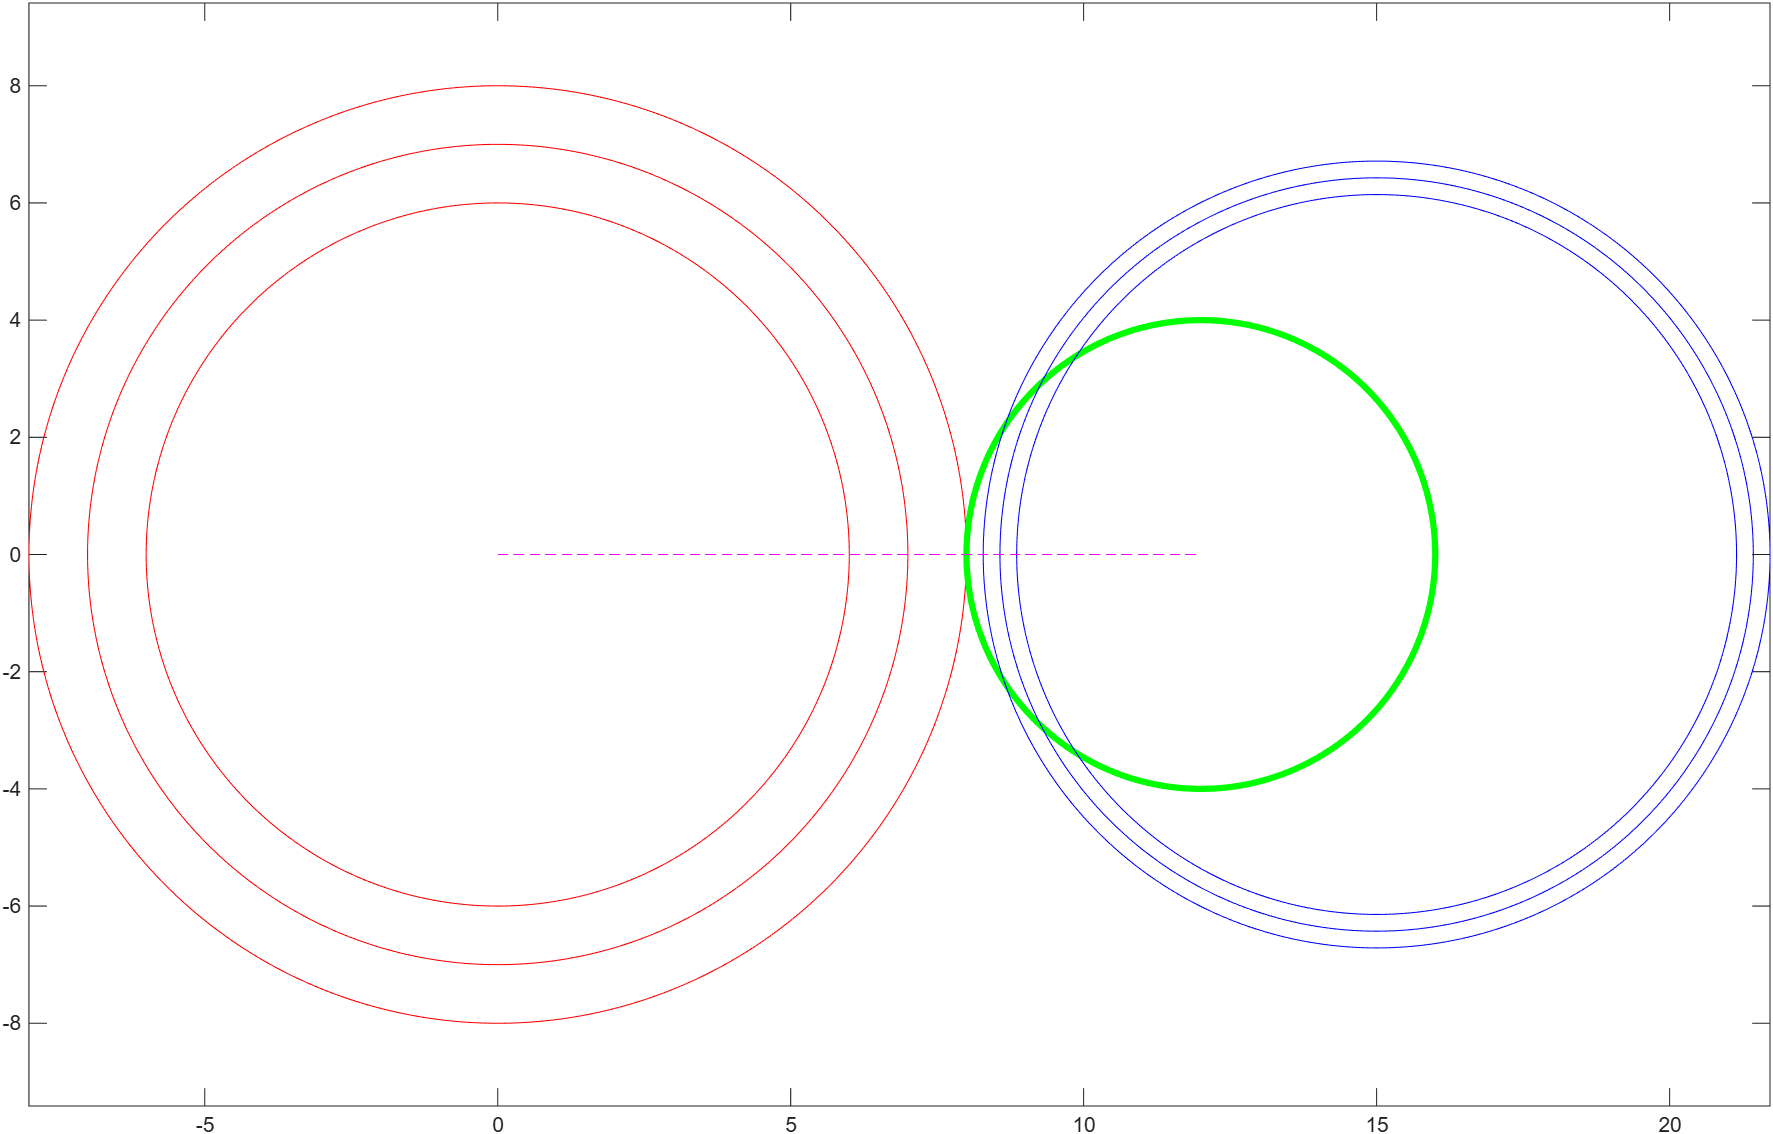
\includegraphics[width=\textwidth]{R1=-8.png}
\textit{(a) $R_1=-8$}
\end{minipage}
\hfill
\begin{minipage}{0.48\textwidth}
\centering
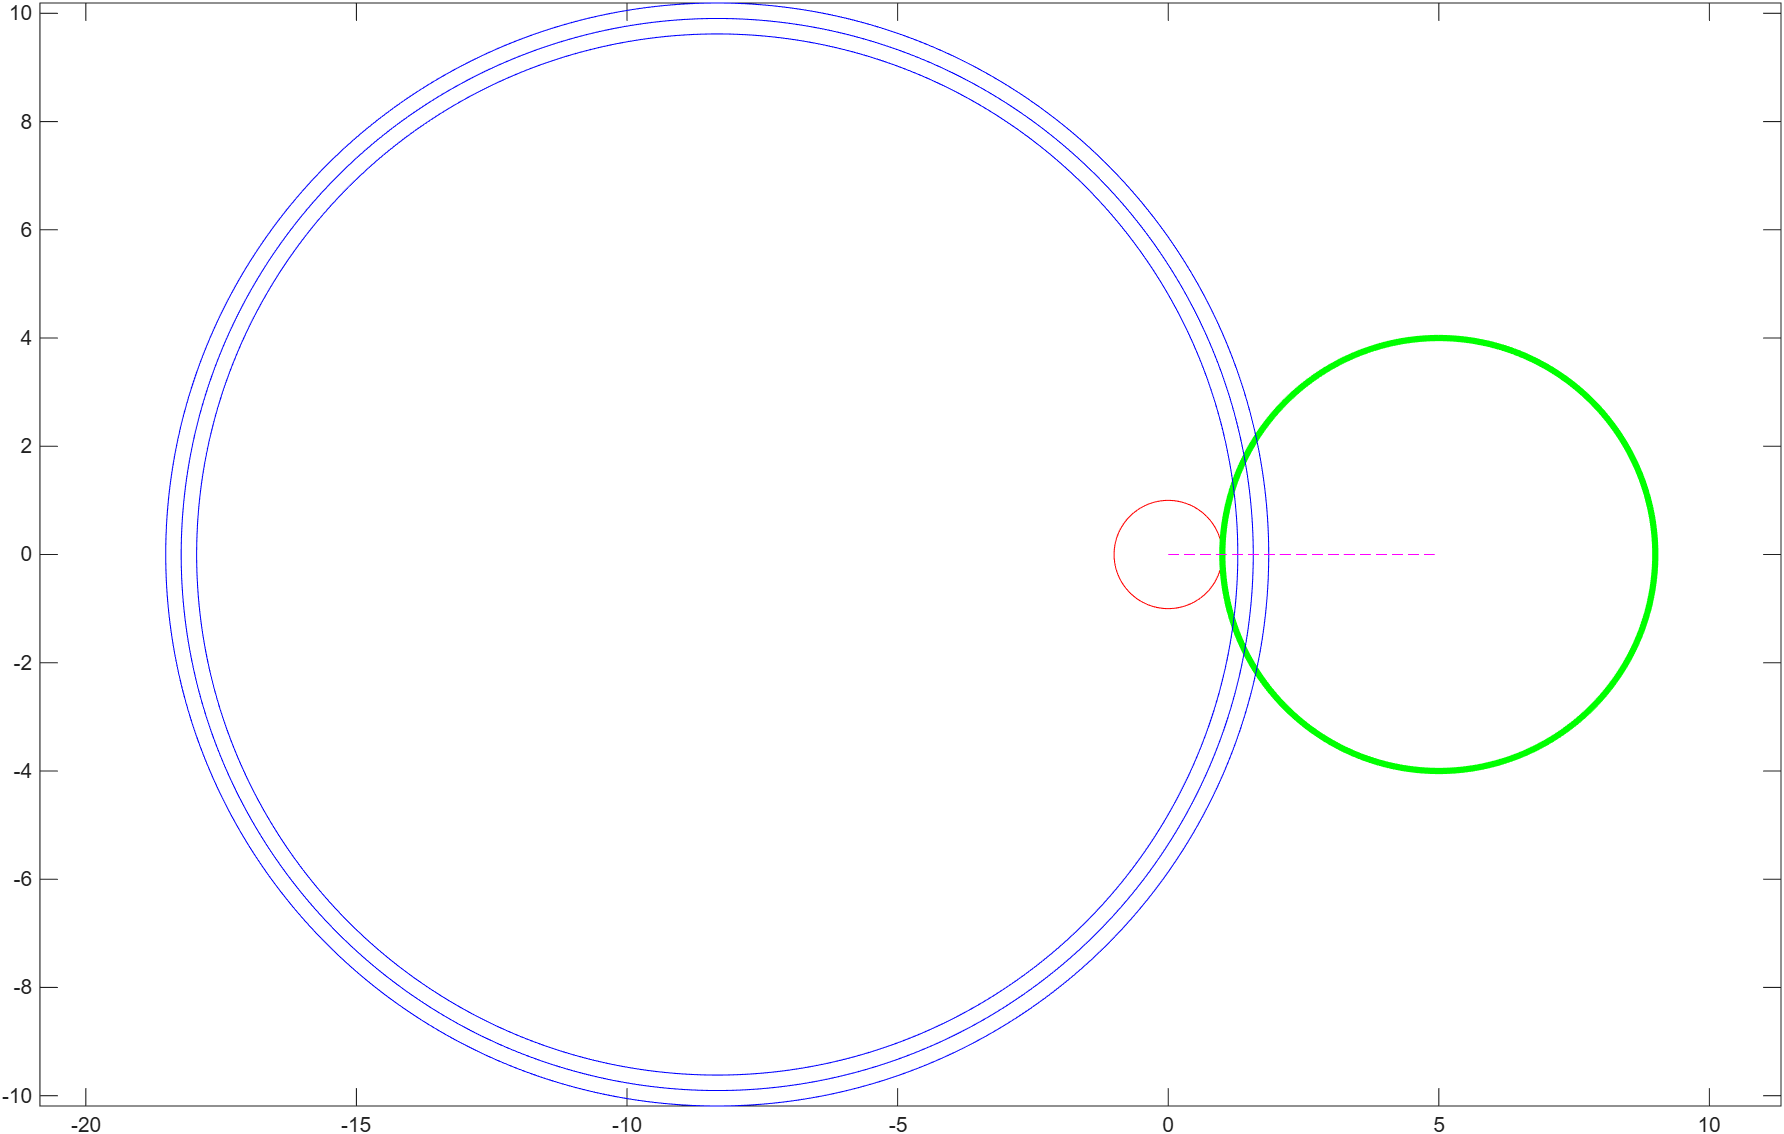
\includegraphics[width=\textwidth]{R1=-1.png}
\textit{(b) $R_1=-1$}
\end{minipage}
\caption{Wpływ krzywizny frontu wejściowego na kształt frontu po przejściu granicy.}
\end{figure}

\subsection{Zmiana promienia krzywizny granicy $R_S$}
\begin{figure}[H]
\centering
\begin{minipage}{0.48\textwidth}
\centering
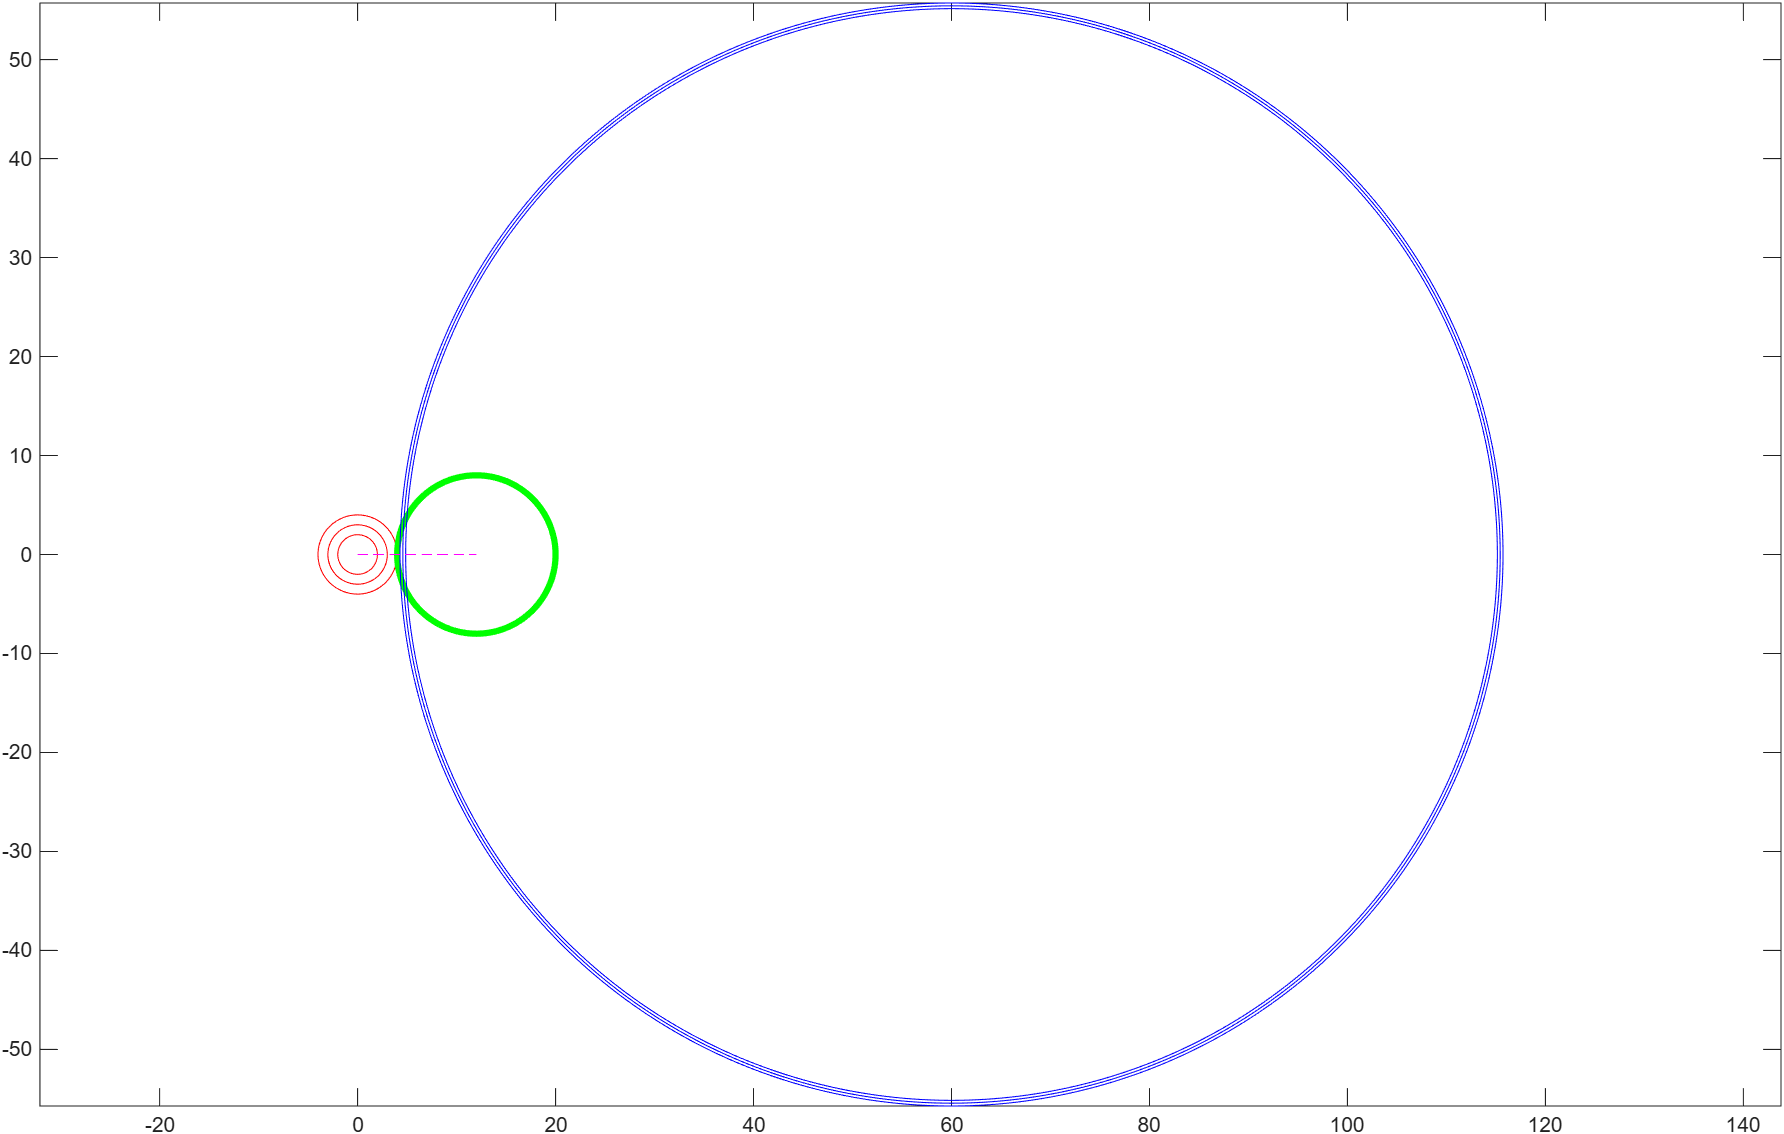
\includegraphics[width=\textwidth]{Rs=8.png}
\textit{(a) $R_S=8$}
\end{minipage}
\hfill
\begin{minipage}{0.48\textwidth}
\centering
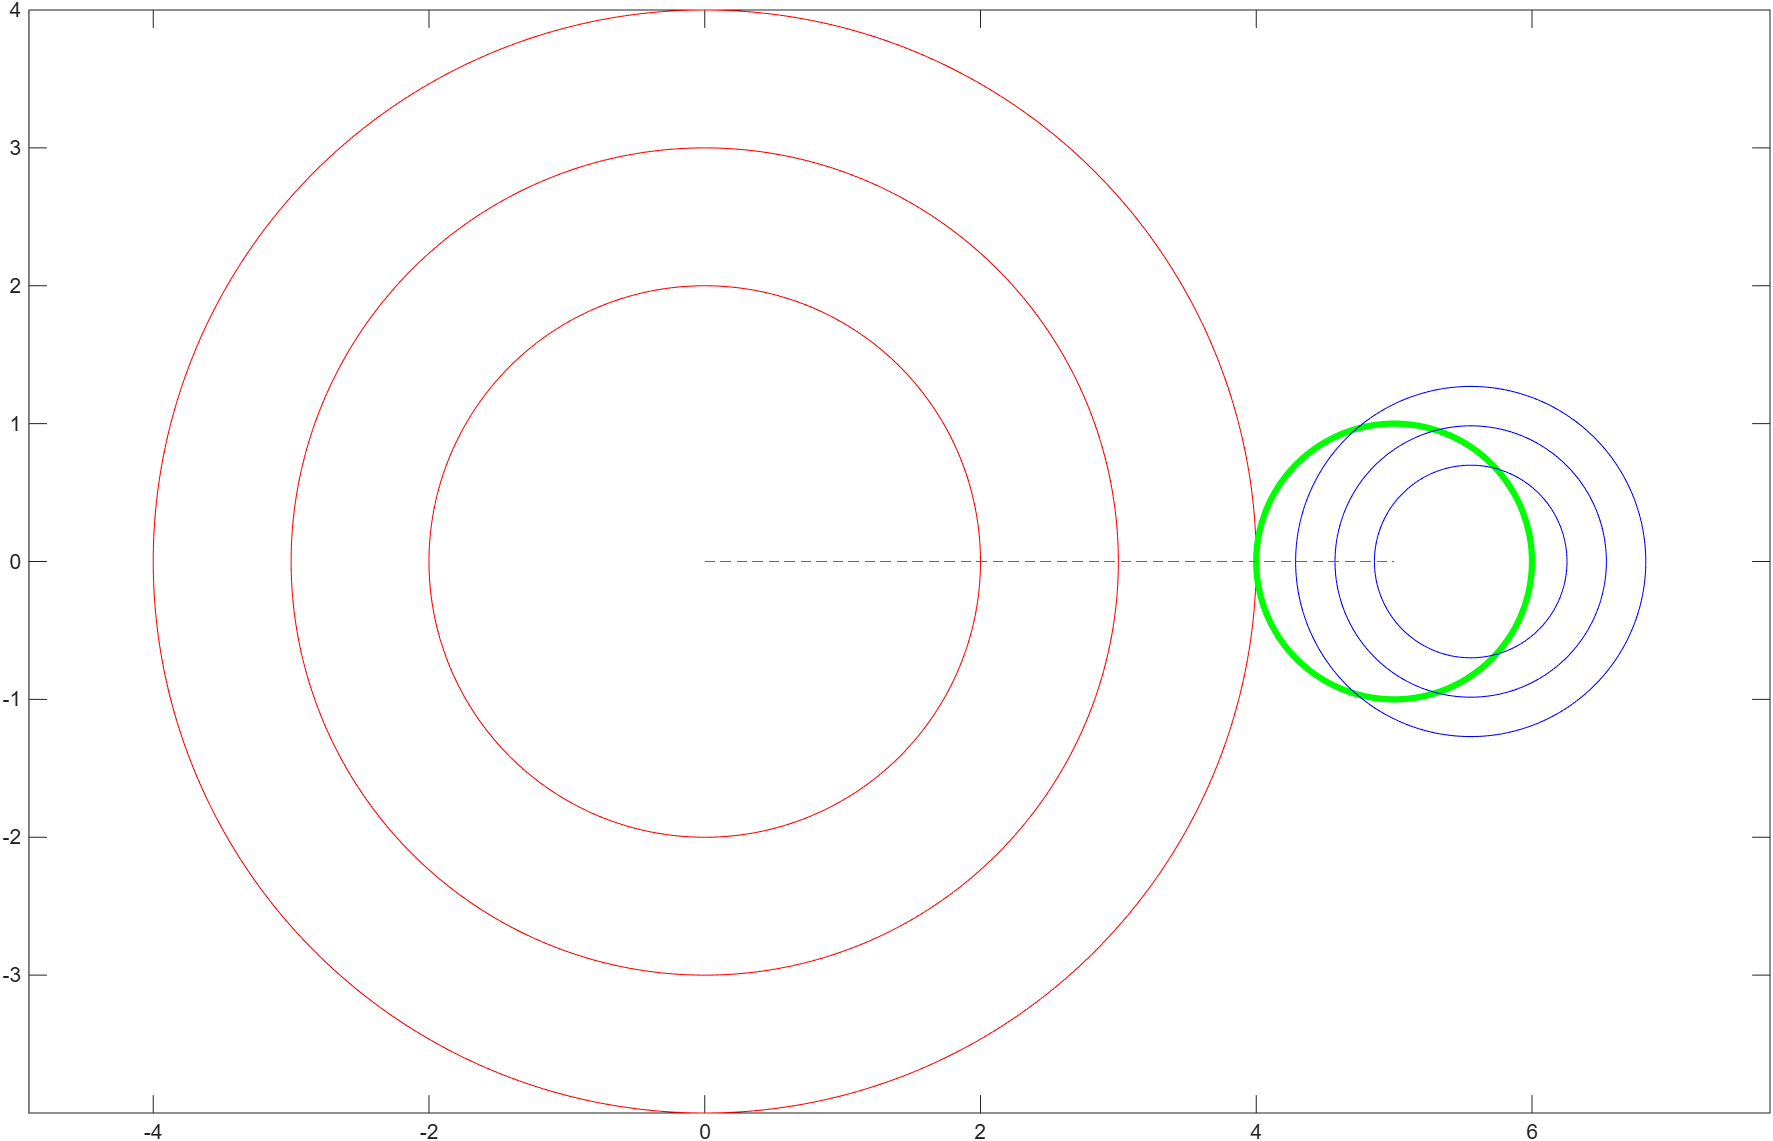
\includegraphics[width=\textwidth]{Rs=1.png}
\textit{(b) $R_S=1$}
\end{minipage}
\caption{Wpływ krzywizny granicy na zmianę krzywizny frontu w ośrodku 2.}
\end{figure}

\section{Wnioski}
\begin{itemize}
\item Zwiększenie długości fali $\lambda$ powoduje proporcjonalne zwiększenie odstępu
między kolejnymi frontami falowymi w obu ośrodkach, bez zmiany ich krzywizny.
\item Większy współczynnik załamania $n$ zwiększa moc optyczną granicy i powoduje
silniejsze skupianie frontu w ośrodku 2 (mniejszy promień $R_2$) oraz mniejszy
odstęp między frontami ($\lambda/n$).
\item Zmniejszanie modułu $|R_1|$ oznacza bardziej zbieżny front wejściowy, co skutkuje
silniejszą zmianą krzywizny po przejściu granicy zgodnie z zależnością
$R_2 = n R_1/(1 + D R_1)$.
\item Mniejszy promień granicy $R_S$ (bardziej wypukła powierzchnia) zwiększa moc
optyczną $D$ i prowadzi do bardziej zbieżnych frontów w ośrodku 2.
\item Przy przejściu sferycznego frontu przez sferyczną granicę krzywizna zmienia się
zgodnie ze wzorem $\tfrac{n_2}{R_2} = \tfrac{n_1}{R_1} + \tfrac{n_2-n_1}{R_S}$. Granica
płaska nie zmienia krzywizny, natomiast granica skupiająca zwiększa zbieżność
frontu. Zmienia się także gęstość frontów wraz ze zmianą długości fali w ośrodku.
\end{itemize}

\end{document}
